\documentclass[
paper=a4,                       % paper size
fontsize=11pt,                  % font size
twoside,                        % two sided
footsepline,                    % add a line to separate the footer
headsepline,                    % add a line to separate the header
headinclude=false,              % header does not belong to the text
footinclude=false,              % footer does not belong to the text
pagesize,                       % set the pagesize in a DVI document
]{scrartcl}

% Copyright (C) 2010,2011,2012 The ESPResSo project
% Copyright (C) 2002,2003,2004,2005,2006,2007,2008,2009,2010
%  Max-Planck-Institute for Polymer Research, Theory Group
%  
% This file is part of ESPResSo.
%   
% ESPResSo is free software: you can redistribute it and/or modify it
% under the terms of the GNU General Public License as published by the
% Free Software Foundation, either version 3 of the License, or (at your
% option) any later version.
%  
% ESPResSo is distributed in the hope that it will be useful, but
% WITHOUT ANY WARRANTY; without even the implied warranty of
% MERCHANTABILITY or FITNESS FOR A PARTICULAR PURPOSE.  See the GNU
% General Public License for more details.
%  
% You should have received a copy of the GNU General Public License
% along with this program.  If not, see <http://www.gnu.org/licenses/>.
%
\usepackage[draft]{varioref}    % defines \vref
\usepackage{hyperref}           % automatically creates links when
                                % using pdflatex, defines \url
\usepackage{ifpdf}              % defines \ifpdf
\usepackage{graphicx}           % handles graphics
\usepackage{color}              % use colors

\usepackage{amsmath}

\usepackage{verbatim}           % required for \verbatim and \endverbatim
\usepackage{fancyvrb}
\usepackage{calc}               % compute length
\usepackage{ifthen}             % provide ifthen
\usepackage{xspace}
\usepackage{units}
\usepackage[numbers]{natbib}

% For building the distribution docs, disable todo boxes.
%\usepackage[disable]{todonotes}
\usepackage{todonotes}

\newcommand{\es}{\mbox{\textsf{ESPResSo}}\xspace}
\newcommand{\ie}{\textit{i.e.}\xspace}
\newcommand{\eg}{\textit{e.g.}\xspace}
\newcommand{\etal}{\textit{et al.}\xspace}

\newcommand{\codebox}[1]%
{\texttt{#1}}

\DefineVerbatimEnvironment{code}{Verbatim}%
{commandchars=\\\{\}}
\makeatletter
\newenvironment{tclcode}
{%
  \addtolength{\linewidth}{-2em}% set the line length
  \@minipagetrue%%%DPC%%%
  \@tempswatrue%%%DPC%%%
  \hsize=\linewidth%
  \setbox0=\vbox\bgroup\verbatim
}{\endverbatim
  \unskip\setbox0=\lastbox%%%DPC%%%
  \egroup
  \par%
  \noindent\hspace{1em}%
  \codebox{\box0}%
  \par\noindent%
}
\makeatother

% \newcommand{\todo}[1]{
%   \marginpar{%
%     \setlength{\fboxrule}{1pt}
%     \fcolorbox{red}{yellow}{%
%       \parbox{\marginparwidth-2\fboxrule-2\fboxsep}{%
%         \bf\raggedright\scriptsize #1%
%       }%
%     }%
%   }%
% }

\makeatletter
\renewcommand{\minisec}[1]{\@afterindentfalse \vskip 1.5ex
  {\parindent \z@
    \raggedsection\normalfont\sffamily\itshape\nobreak#1\par\nobreak}%
  \@afterheading}
\makeatother

\newcommand{\esptitlehead}{
  \titlehead{
    \begin{center}
      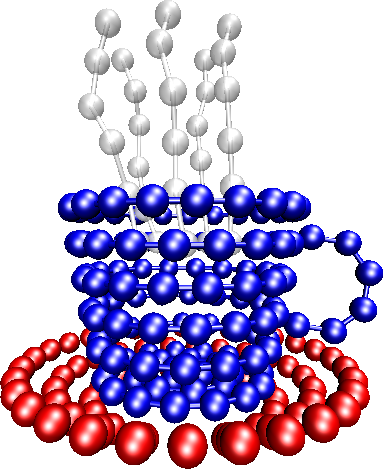
\includegraphics[width=5cm]{logo/transparentbg}
    \end{center}
  }
}

\usepackage{graphicx}
\usepackage{verbatim}

\newtheorem{task}{Task}

\begin{document}

\esptitlehead

\title{Tutorial 8: Visualization%
\ifdefined\esversion%
\thanks{For \es \esversion}%
\fi%
}
\subtitle{How to visualize your \es simulations while they are running}
\maketitle

\section{Introduction}
\label{intro}

When you are running a simulation, it is often useful to see what is going on by visualizing particles in a 3D view or by plotting observables over time.
That way, you can easily determine things like whether your choice of parameters has led to a stable simulation or whether your system has equilibrated.
You may even be able to do your complete data analysis in real time as the simulation progresses.\\

\noindent Thanks to \es's Python interface, we can make use of standard libraries like Mayavi or OpenGL (for interactive 3D views) and Matplotlib (for line graphs) for this purpose.
We will also use NumPy, which both of these libraries depend on, to store data and perform some basic analysis.

\section{Simulation}
\label{sim}

First, we need to set up a simulation.
We simulate a simple Lennard-Jones liquid in this tutorial using the script shown below.

\pypressoexternal{scripts/simulation.py}

\section{Live plotting}
\label{plot}

Let's have a look at the total energy of the simulation.
We can determine the individual energies in the system using
\begin{pypresso}
print (system.analysis.energy())
\end{pypresso}
to get
\begin{pypresso}
OrderedDict([
        ('total', 1840.118038871784),
        ('ideal', 1358.743742464325),
        ('bonded', 0.0), 
        (('nonBonded', 0, 0), 481.374296407459), 
        ('nonBonded', 481.374296407459), 
        ('coulomb', 0.0)])
\end{pypresso}
Write that command right after the call to \pypressoinline{main()} and see if you can get a similar result.
Now we want to store the total energy over time in a NumPy array.
To do that, modify the \pypressoinline{main} function definition to be the following:
\begin{pypresso}
energies = numpy.empty((int_steps,2))
def main():
    for i in range(0, int_n_times):
        print("run %d at time=%f " % (i, system.time))
        system.integrator.run(int_steps)
        energies[i] = (system.time, system.analysis.energy()['total'])
\end{pypresso}
Now we can do some analysis on the stored energies.
For example, let us calculate the time-averaged energy:
\begin{pypresso}
print ("Average energy: %.6g" % energies[:,1].mean())
\end{pypresso}
We can also plot the energy over time by adding
\begin{pypresso}
pyplot.xlabel("time")
pyplot.ylabel("energy")
pyplot.plot(energies[:,0],energies[:,1])
pyplot.show()
\end{pypresso}
to the end of the script. Of course, this plot only gets shown after the entire simulation is completed.
To get an interactive plot, we update it from within the integration loop.
\begin{pypresso}
energies = numpy.empty((int_steps,2))
current_time = -1
pyplot.xlabel("time")
pyplot.ylabel("energy")
plot, = pyplot.plot([0],[0])
pyplot.show(block=False)
def update_plot():
    if current_time < 0:
        return
    i = current_time
    plot.set_xdata(energies[:i+1,0])
    plot.set_ydata(energies[:i+1,1])
    pyplot.xlim(0, energies[i,0])
    pyplot.ylim(energies[:i+1,1].min(), energies[:i+1,1].max())
    pyplot.draw()
    pyplot.pause(0.01)
def main():
    global current_time
    for i in range(0, int_n_times):
        print("run %d at time=%f " % (i, system.time))
        system.integrator.run(int_steps)
        energies[i] = (system.time, system.analysis.energy()['total'])
        current_time = i
        update_plot()
\end{pypresso}

\noindent One shortcoming of this simple method is that one cannot interact with the controls of the plot window (e.g. resize the window or zoom around in the graph).
This will be resolved using multiple threads when we combine the plotting with the 3D visualization in the next section.

\section{Live visualization}
\label{vis}

In order to be able to interact with the live visualization, we need to move the main integration loop into a secondary thread and run the visualization in the main thread (note that visualization or plotting cannot be run in secondary threads). First, let's revert to the main loop without plotting:
\begin{pypresso}
energies = numpy.empty((int_steps,2))
def main():
    for i in range(0, int_n_times):
        print("run %d at time=%f " % (i, system.time))
        system.integrator.run(int_steps)
        energies[i] = (system.time, system.analysis.energy()['total'])
\end{pypresso}

Then, add the following line after the particle setup code:
\begin{pypresso}
visualizer = visualization.openGLLive(system)
\end{pypresso}
Now, go to the end of the \pypressoinline{main} function definition and add
\begin{pypresso}
visualizer.update()
\end{pypresso}
which sends the current simulation state to the visualizer.
Now, go to the line where \pypressoinline{main()} is called and replace it with the following code, which dispatches the function in a secondary thread, and then opens the visualizer window:
\begin{pypresso}
t = Thread(target=main)
t.daemon = True
t.start()
visualizer.start()
\end{pypresso}

To follow the trajectories, try decreasing the integration steps to 1 and the
time step to 0.001.  While the simulation is running, you can move and zoom
around with your mouse. Alternatively, you can try mayavi by
switching the visualizer to:

\begin{pypresso}
visualizer = visualization.mayaviLive(system)
\end{pypresso}

In mayavi, explore the buttons in the toolbar to see how the graphical representation can be changed

\section{Combined live visualization and plotting}

Now let's merge the code from the preceding two sections so we can see the energy graph while viewing the 3D visualization of the particles.
Do do that, we copy the \pypressoinline{pyplot}-related lines from above:

\begin{pypresso}
current_time = -1
pyplot.xlabel("time")
pyplot.ylabel("energy")
plot, = pyplot.plot([0],[0])
pyplot.show(block=False)
def update_plot():
    if current_time < 0:
        return
    i = current_time
    plot.set_xdata(energies[:i+1,0])
    plot.set_ydata(energies[:i+1,1])
    pyplot.xlim(0, energies[i,0])
    pyplot.ylim(energies[:i+1,1].min(), energies[:i+1,1].max())
    pyplot.draw()
    pyplot.pause(0.01)
\end{pypresso}

Then we merge the \pypressoinline{main} function definitions from both the previous sections.

\begin{pypresso}
def main():
    global current_time
    for i in range(0, int_n_times):
        print("run %d at time=%f " % (i, system.time))
        system.integrator.run(int_steps)
        energies[i] = (system.time, system.analysis.energy()['total'])
        current_time = i
        visualizer.update()
        # update_plot() cannot be called from here
\end{pypresso}

However, as we now have multiple threads, we cannot simply call \pypressoinline{update_plot()} from the \pypressoinline{main} function definition.
Instead, we register it as a callback with the visualizer before we start up the visualizer GUI:

\begin{pypresso}
t = Thread(target=main)
t.daemon = True
t.start()
visualizer.register_callback(update_plot, interval=500)
visualizer.start()
\end{pypresso}

\section{Customizing the OpenGL visualizer}

Visualization of more advanced features of \es is also possible (e.g.
bonds, constraints and lattice Boltzmann velicity fields) with the OpenGL
visualizer. There are a number of optional keywords that can be used to specify the
appearance of the visualization, they are simply stated after
\pypressoinline{system} when creating the visualizer instance.
See the following examples:

\begin{pypresso} 
# Enables particle dragging via mouse:
visualizer = visualization.openGLLive(system, drag_enabled=True)
\end{pypresso}

\begin{pypresso} 
# Use a white background:
visualizer = visualization.openGLLive(system, background_color = [1,1,1])
\end{pypresso}

\begin{pypresso} 
# Static, uniform lightning
visualizer = visualization.openGLLive(system, light_pos = system.box_l*2.0, light_brightness = 5.0, spotlight_brightness = 0.0)
\end{pypresso}

The visualizer options are stored in the dict \pypressoinline{visualizer.specs},
the following snippet prints out the current configuration nicely: 

\begin{pypresso} 
for k in sorted(visualizer.specs.keys(), key=lambda s: s.lower()): print("{:30}  {}".format(k, visualizer.specs[k]))
\end{pypresso}

All keywords are explained in the Online Documentation at
\url{http://espressomd.org/html/doc/io.html#opengl-visualizer}.  

\section{Further examples with OpenGL}

There are a number of specific visualization examples for \es and the OpenGL visualizer that can be found
in the \path{samples} folder. You may need to recompile \es with the following features used in the examples:

\begin{pypresso}
#define PARTIAL_PERIODIC
#define EXTERNAL_FORCES
#define CONSTRAINTS
#define MASS
#define NPT
#define ELECTROSTATICS
#define LB
#define LB_BOUNDARIES
#define LENNARD_JONES
\end{pypresso}


\begin{itemize}

\item \path{billard.py} A simple billard game made with \es.

\item \path{visualization_openGL.py} Sample for an opengl visualization with user-defined keyboard- and timed callbacks.

\item \path{visualization_bonded.py} Opengl visualization for bonds.

\item \path{visualization_npt.py} Simple test visualization for the NPT ensemble.

\item \path{visualization_poisseuille.py} Visualization for poisseuille flow with Lattice-Boltzmann.

\item \path{visualization_constraints.py} Constraint visualization with opengl with all avaiable constraints (commented out).

\item \path{visualization_mmm2d.py} A visual sample for a constant potential plate capacitor simulated with mmm2d.

\end{itemize}

\end{document}
